%%%%%%%%%%%%%%%%%%%%%%%%%%%%%%%%%%%%%%%%%%%%%%%%%%%%%%%%%%%%%%%%%%%%%
% Mitschrieb vom 09.01.2014                                         %
%%%%%%%%%%%%%%%%%%%%%%%%%%%%%%%%%%%%%%%%%%%%%%%%%%%%%%%%%%%%%%%%%%%%%
\chapter{Euklidische und nichteuklidische Geometrie}

\begin{definition}
    Das Tripel $(X, d, G)$ heißt genau dann eine \textbf{Geometrie}\xindex{Geometrie},
    wenn $(X, d)$ ein metrischer Raum und $\emptyset \neq G \subseteq \powerset{X}$
    die Menge aller \textbf{Geraden}\xindex{Gerade} ist.
\end{definition}

\section{Axiome für die euklidische Ebene}
Axiome\xindex{Axiom} bilden die Grundbausteine jeder mathematischen Theorie. Eine
Sammlung aus Axiomen nennt man Axiomensystem\xindex{Axiomensystem}.
Da der Begriff des Axiomensystems so grundlegend ist, hat man auch 
ein paar sehr grundlegende Forderungen an ihn: Axiomensysteme sollen
\textbf{widerspruchsfrei} sein, die Axiome sollen möglichst
\textbf{unabhängig} sein und \textbf{Vollständigkeit} wäre auch toll.
Mit Unabhängigkeit ist gemeint, dass kein Axiom sich aus einem anderem
herleiten lässt. Dies scheint auf den ersten Blick eine einfache
Eigenschaft zu sein. Auf den zweiten Blick muss man jedoch einsehen, 
dass das Parallelenproblem, also die Frage ob das Parallelenaxiom 
unabhängig von den restlichen Axiomen ist, über 2000 Jahre nicht 
gelöst wurde. Ein ganz anderes Kaliber ist die Frage nach der
Vollständigkeit. Ein Axiomensystem gilt als Vollständig, wenn
jede Aussage innerhalb des Systems verifizierbar oder falsifizierbar
ist. Interessant ist hierbei der Gödelsche Unvollständigkeitssatz, 
der z.~B. für die Arithmetik beweist, dass nicht alle Aussagen
formal bewiesen oder widerlegt werden können.

Kehren wir nun jedoch zurück zur Geometrie. Euklid hat in seiner 
Abhandlung \enquote{Die Elemente} ein Axiomensystem für die Geometrie
aufgestellt. 

\textbf{Euklids Axiome}
\begin{itemize}
    \item \textbf{Strecke} zwischen je zwei Punkten
    \item Jede Strecke bestimmt genau eine \textbf{Gerade}
    \item \textbf{Kreis} (um jeden Punkt mit jedem Radius)
    \item Je zwei rechte Winkel sind gleich (Isometrie, Bewegung)
    \item Parallelenaxiom von Euklid:\xindex{Parallelenaxiom}\\
        Wird eine Gerade so von zwei Geraden geschnitten, dass die 
        Summe der Innenwinkel zwei Rechte ist, dann schneiden sich
        diese Geraden auf der Seite dieser Winkel.\\
        \\
        Man mache sich klar, dass das nur dann nicht der Fall ist, 
        wenn beide Geraden parallel sind und senkrecht auf die erste stehen.
\end{itemize}

\begin{definition}\xindex{Ebene!euklidische}%In Vorlesung: Definition 14.2
    Eine \textbf{euklidische Ebene} ist ein metrischer Raum $(X,d)$ 
    zusammen mit einer Teilmenge $\emptyset \neq G \subseteq \powerset{X}$, sodass die
    Axiome~\ref{axiom:1}~-~\ref{axiom:4} erfüllt sind:
    \begin{enumerate}[label=§\arabic*),ref=§\arabic*]
        \item \textbf{Inzidenzaxiome}\xindex{Inzidenzaxiome}:\label{axiom:1}
            \begin{enumerate}[label=(\roman*),ref=\theenumi{} (\roman*)]
                \item \label{axiom:1.1} Zu $P \neq Q \in X$ gibt es genau ein $g \in G$ mit
                      $\Set{P, Q} \subseteq g$.
                \item \label{axiom:1.2} $|g| \geq 2 \;\;\; \forall g \in G$
                \item \label{axiom:1.3} $X \notin G$
            \end{enumerate}
        \item \textbf{Abstandsaxiom}\xindex{Abstandsaxiom}: Zu $P, Q, R \in X$ gibt es \label{axiom:2}
              genau dann ein $g \in G$ mit $\Set{P, Q, R} \subseteq g$,
              wenn gilt: 
              \begin{itemize}[]
                \item $d(P, R) = d(P, Q) + d(Q, R)$ oder
                \item $d(P, Q) = d(P, R) + d(R, Q)$ oder
                \item $d(Q, R) = d(Q, P) + d(P, R)$
              \end{itemize}
    \end{enumerate}
\end{definition}

\begin{definition}
    \begin{defenum}
        \item $P, Q, R$ liegen \textbf{kollinear}\xindex{kollinear}, 
              wenn es $g \in G$ gibt mit $\Set{P, Q, R} \subseteq g$.
        \item $Q$ \textbf{liegt zwischen}\xindex{liegt zwischen} $P$
              und $R$, wenn $d(P, R) = d(P, Q) + d(Q, R)$
        \item \textbf{Strecke}\xindex{Strecke} $\overline{PR} := \Set{Q \in X | Q \text{ liegt zwischen } P \text{ und } R}$
        \item \textbf{Halbgeraden}\xindex{Halbgerade}:\\
              $PR^+ := \Set{Q \in X | Q \text{ liegt zwischen } P \text{ und } R \text{ oder } R \text{ liegt zwischen } P \text{ und } Q}$\\
              $PR^- := \Set{Q \in X | P \text{ liegt zwischen } Q \text{ und } R}$\\ 
    \end{defenum}
\end{definition}

\begin{figure}[htp]
    \centering
    \documentclass[varwidth=true, border=2pt]{standalone}
\usepackage{tikz}
\usetikzlibrary{snakes}

\begin{document}
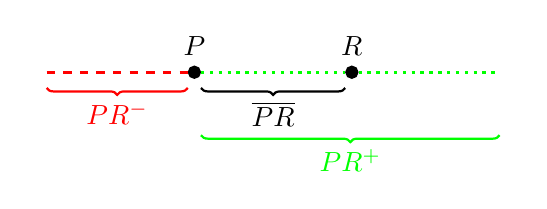
\begin{tikzpicture}
    \tikzstyle{point}=[circle,thick,draw=black,fill=black,inner sep=0pt,minimum width=4pt,minimum height=4pt]
    \node (Pleft) at (0,0) {};
    \node (P)[point,label=90:$P$] at (2,0) {};
    \node (R)[point,label=90:$R$] at (4,0) {};
    \node (Rright) at (6,0) {};
    \draw[red,dashed,very thick] (Pleft) -- (P);
    \draw[green,dotted,very thick] (P) -- (R) -- (Rright);
    \draw [thick,decoration={brace,mirror,raise=0.2cm},decorate,red] (Pleft) -- (P) node [pos=0.5,anchor=north,yshift=-0.25cm,red] {$PR^-$}; 
    \draw [thick,decoration={brace,mirror,raise=0.2cm},decorate] (P) -- (R) node [pos=0.5,anchor=north,yshift=-0.25cm] {$\overline{PR}$}; 
    \draw [thick,decoration={brace,mirror,raise=0.8cm},decorate,green] (P) -- (Rright) node [pos=0.5,anchor=north,yshift=-0.85cm,green] {$PR^+$}; 
\end{tikzpicture}
\end{document}

    \caption{Halbgeraden}
    \label{fig:halbgeraden}
\end{figure}

\begin{bemerkung}
    \begin{bemenum}
        \item $PR^+ \cup PR^- = PR$
        \item $PR^+ \cap PR^- = \Set{P}$
    \end{bemenum}
\end{bemerkung}

\begin{beweis}\leavevmode
    \begin{enumerate}[label=(\roman*)]
        \item \enquote{$\subseteq$} folgt direkt aus der Definition von $PR^+$ und $PR^-$\\
              \enquote{$\supseteq$}: Sei $Q \in PR \Rightarrow P, Q, R$ 
              sind kollinear.\\
              $\overset{\ref{axiom:2}}{\Rightarrow}
              \begin{cases} 
                Q \text{ liegt zwischen } P \text{ und } R \Rightarrow Q \in PR\\
                R \text{ liegt zwischen } P \text{ und } Q \Rightarrow Q \in PR\\
                P \text{ liegt zwischen } Q \text{ und } R \Rightarrow Q \in PR
              \end{cases}$
        \item \enquote{$\supseteq$} ist offensichtlich\\
              \enquote{$\subseteq$}: Sei $PR^+ \cap PR^-$. Dann ist
              $d(Q,R) = d(P,Q) + d(P,R)$ weil $Q \in PR^-$ und
              \begin{align*}
                &\left \{ \begin{array}{l}
                        d(P,R) = d(P,Q) + d(Q,R) \text{ oder }\\
                        d(P,Q) = d(P,R) + d(R,Q)
                       \end{array} \right \}\\
                &\Rightarrow d(Q,R) = 2d(P,Q) + d(Q,R)\\
                &\Rightarrow d(P,Q) = 0\\
                &\Rightarrow P=Q\\
                &d(P,Q) = 2d(P,R) + d(P,Q)\\
                &\Rightarrow P=R\\
                &\Rightarrow \text{Widerspruch}
              \end{align*}
    \end{enumerate}
\end{beweis}

\begin{definition}
    \begin{enumerate}[label=§\arabic*),ref=§\arabic*,start=3]
        \item \label{axiom:3}\textbf{Anordnungsaxiome}\xindex{Anordnungsaxiome}
            \begin{enumerate}[label=(\roman*),ref=\theenumi{} (\roman*)]
                \item \label{axiom:3.1} Zu jedem $P \in X$ jeder 
                      Halbgerade $H$ mit Anfangspunkt $P$ und jedem 
                      $r \in \mdr_{\geq 0}$ gibt es genau ein 
                      $Q \in H$ mit $d(P,Q) = r$.
                \item \label{axiom:3.2} Jede Gerade zerlegt 
                      $X \setminus g = H_1 \dcup H_2$ in zwei 
                      nichtleere Teilmengen $H_1, H_2$,
                      sodass für alle $A \in H_i$, $B \in H_j$ mit
                      $i,j \in \Set{1,2}$ gilt: 
                      $\overline{AB} \cap g \neq \emptyset \Leftrightarrow i \neq j$.\\
                      Diese Teilmengen $H_i$ heißen 
                      \textbf{Halbebenen}\xindex{Halbebene} bzgl. 
                      $g$.
            \end{enumerate}
        \item \label{axiom:4}\textbf{Bewegungsaxiom}\xindex{Bewegungsaxiom}: Zu $P, Q, P', Q' \in X$
            mit $d(P,Q) = d(P', Q')$. Isometrien $\varphi_1, \varphi_2$
            mit $\varphi_i (P) = P'$ und $\varphi_i(Q) = Q', i=1,2$
            (Spiegelung an der Gerade durch $P$ und $Q$ ist nach 
             Identifizierung von $P \cong P'$ und $Q \cong Q'$ eine
             weitere Isometrie.)
        \item \label{axiom:5}\textbf{Parallelenaxiom}: Für jedes $g \in G$ und jedes
            $P \in X \setminus g$ gibt es höchstens ein $h \in G$ mit
            $h \cap g = \emptyset$.\footnote{$h$ heißt \enquote{Parallele zu $g$ durch $P$}.}
    \end{enumerate}
\end{definition}

%%%%%%%%%%%%%%%%%%%%%%%%%%%%%%%%%%%%%%%%%%%%%%%%%%%%%%%%%%%%%%%%%%%%%
% Mitschrieb vom 14.01.2014                                         %
%%%%%%%%%%%%%%%%%%%%%%%%%%%%%%%%%%%%%%%%%%%%%%%%%%%%%%%%%%%%%%%%%%%%%
\begin{satz}[Satz von Pasch]\label{satz:pasch} %In Vorlesung: Bemerkung 14.5
    Seien $P$, $Q$, $R$ nicht kollinear, $g \in G$ mit $g \cap \Set{P, Q, R} = \emptyset$
    und $g \cap \overline{PQ} \neq \emptyset$. 

    Dann ist entweder $g \cap \overline{PR} \neq \emptyset$ oder 
                      $g \cap \overline{QR} \neq \emptyset$.
\end{satz}

Dieser Satz besagt, dass Geraden, die eine Seite eines Dreiecks 
(also nicht nur eine Ecke) schneiden, auch eine weitere Seite 
scheiden.

\begin{beweis}
    $g \cap \overline{PQ} \neq \emptyset$\\
    $\overset{\mathclap{\ref{axiom:3.2}}}{\Rightarrow} P$ und $Q$ liegen in verschiedenen Halbebenen bzgl. $g$\\
    $\Rightarrow$ \obda $R$ und $P$ liegen in verschieden
    Halbebenen bzgl. $g$\\
    $\Rightarrow g \cap \overline{RP} \neq \emptyset$
\end{beweis}

\begin{bemerkung}\label{kor:beh3}
    Sei $P, Q \in X$ mit $P \neq Q$ sowie $A, B \in X \setminus PQ$ 
    mit $A \neq B$.
    Außerdem seien $A$ und $B$ in der selben Halbebene bzgl. $PQ$ sowie
    $Q$ und $B$ in der selben Halbenebe bzgl. $PA$.

    Dann gilt: $PB^+ \cap \overline{AQ} \neq \emptyset$
\end{bemerkung}

\begin{figure}[htp]
    \centering
    \usetkzobj{all}
\begin{tikzpicture}
    \tkzSetUpPoint[shape=circle,size=10,color=black,fill=black]
    \tkzSetUpLine[line width=1]
    \tkzDefPoints{0/0/P, 4/1/Q, 2/3/A, 5/3/B}
    \tkzInterLL(P,B)(A,Q) \tkzGetPoint{C}
    \tkzDrawPoints(P,Q,A,B,C)

    %\tkzDrawSegments(P,Q Q,A A,P)
    %\tkzDrawSegments[dashed](P,B B,Q)
    \tkzDrawLine(P,Q)
    \tkzDrawLine(P,A)
    \tkzDrawLine(A,Q)
    \tkzDrawLine(P,B)


    \tkzLabelPoint[below](P){$P$}
    \tkzLabelPoint[below](Q){$Q$}
    \tkzLabelPoint[below](A){$A$}
    \tkzLabelPoint[below](B){$B$}
    \tkzLabelPoint[above](C){$C$}
\end{tikzpicture}

    \caption{Situation aus \cref{kor:beh3}}
    \label{fig:bild-5}
\end{figure}

Auch \cref{kor:beh3} lässt sich Umgangssprachlich sehr viel 
einfacher ausdrücken: Die Diagonalen eines konvexen Vierecks 
schneiden sich.

\begin{beweis}%In Vorlesung: Behauptung 3
    Sei $P' \in PQ^-, P' \neq P$
    $\overset{\cref{satz:pasch}}{\Rightarrow} PB$ schneidet
    $\overline{AP'} \cup \overline{AQ}$

    Sei $C$ der Schnittpunkt. Dann gilt:
    \begin{enumerate}[label=(\roman*)]
        \item $C \in PB^+$, denn $A$ und $B$ liegen in derselben
              Halbebene bzgl. $PQ = P'Q$, also auch
              $\overline{AP'}$ und $\overline{AQ}$.
        \item $C$ liegt in derselben Halbebene bzgl. $PA$ wie
              $B$, weil das für $Q$ gilt.

              $\overline{AP'}$ liegt in der anderen Halbebene
              bzgl. $PA \Rightarrow C \notin \overline{P'A} \Rightarrow C \in \overline{AQ}$
    \end{enumerate}
    Da $C \in PB^+$ und $C \in \overline{AQ}$ folgt nun direkt: 
    $\emptyset \neq \Set{C} \subseteq PB^+ \cap \overline{AQ} \qed$
\end{beweis}

\begin{bemerkung}\label{kor:14.6}%In Vorlesung: Bemerkung 14.6
    Seien $P, Q \in X$ mit $P \neq Q$ und $A, B \in X \setminus PQ$
    in der selben Halbebene bzgl. $PQ$. Außerdem sei $d(A,P)=d(B,P)$
    und $d(A, Q) = d(B, Q)$.

    Dann ist $A = B$.
\end{bemerkung}

\begin{figure}[htp]
    \centering
    \begin{tikzpicture}
    \tikzstyle{point}=[circle,thick,draw=black,fill=black,inner sep=0pt,minimum width=4pt,minimum height=4pt]
    \node (P)[point,label={[label distance=0cm]-90:$P$}] at (0,0) {};
    \node (Q)[point,label={[label distance=0cm]-90:$Q$}] at (5,1) {};
    \node (A)[point,label={[label distance=0cm]180:$A$}] at (2,2) {};
    \node (B)[point,label={[label distance=0cm]190:$B$}] at (1,3) {};

    \draw[very thick] (P) edge node  {} (Q);
    \draw[very thick, red] (P) edge node {} (A);
    \draw[very thick, red] (P) edge node {} (B);
    \draw[very thick, blue] (Q) edge node {} (A);
    \draw[very thick, blue] (Q) edge node {} (B);

    \draw[very thick] ($(P)!-1cm!(Q)$) -- ($(Q)!-1cm!(P)$);
\end{tikzpicture}

    \caption{\cref{kor:14.6}: Die beiden roten und die beiden blauen Linien sind gleich lang. Intuitiv weiß man, dass daraus folgt, dass $A = B$ gilt.}
    \label{fig:bild-2}
\end{figure}

\begin{beweis} durch Widerspruch\\
    \underline{Annahme}: $A \neq B$

    Dann ist $B \notin (PA \cup QA)$ wegen \ref{axiom:2}.

    \begin{figure}[ht]
        \centering
        \subfloat[1. Fall]{
            \begin{tikzpicture}
    \tkzSetUpPoint[shape=circle,size=10,color=black,fill=black]
    \tkzSetUpLine[line width=1]
    \tkzDefPoints{0/0/P, 4/0/Q, 1/0.5/B, 1/2/A}
    \tkzInterLL(P,B)(Q,A) \tkzGetPoint{C}

    \tkzDrawLine(P,A)
    \tkzDrawLine(Q,A)
    \tkzDrawLine(P,Q)
    \tkzDrawLine[add=0 and 0.5](P,C)
    \tkzDrawSegments(B,Q)

    \tkzDrawPoints(P,Q,B,C,A)
    \tkzLabelPoint[below](P){$P$}
    \tkzLabelPoint[below](Q){$Q$}
    \tkzLabelPoint[below](B){$B$}
    \tkzLabelPoint[below](C){$C$}
    \tkzLabelPoint[below](A){$A$}
\end{tikzpicture}

            \label{fig:bild-3}
        }%
        \subfloat[2. Fall]{
            \begin{tikzpicture}
    \tkzSetUpPoint[shape=circle,size=10,color=black,fill=black]
    \tkzSetUpLine[line width=1]
    \tkzDefPoints{0/0/P, 4/1/Q, 2/3/A, 0/3/B}

    \tkzDrawSegments(P,Q Q,A A,P)
    \tkzDrawSegments[dashed](P,B B,Q)
    \tkzDrawLine(P,Q)

    \tkzDrawPoints(P,Q,A,B)
    \tkzLabelPoint[below](P){$P$}
    \tkzLabelPoint[below](Q){$Q$}
    \tkzLabelPoint[above](A){$A$}
    \tkzLabelPoint[above](B){$B$}
\end{tikzpicture}

            \label{fig:bild-4}
        }%
        \label{Formen}
        \caption{Fallunterscheidung aus \cref{kor:14.6}}
    \end{figure}

    \underline{1. Fall}: $Q$ und $B$ liegen in derselben Halbebene bzgl. $PA$

    $\overset{\cref{kor:beh3}}{\Rightarrow} PB^+ \cap \overline{AQ} \neq \emptyset$.

    Sei $C$ der Schnittpunkt vom $PB$ und $AQ$.

    Dann gilt:
    \begin{enumerate}[label=(\roman*)]
        \item $d(A, C) + d(A, Q) = d(B, Q) < d(B, C) + d(C, Q) \Rightarrow d(A, C) < d(B, C)$ \label{enum:komischer-beweis-i}
        \item \begin{enumerate}[label=\alph*)]
                \item $B$ liegt zwischen $P$ und $C$.

                      $d(P,A) + d(A, C) > d(P,C) = d(P,B) + d(B,c) = d(P,A) + d(B,C)$
                      $\Rightarrow d(A,c) > d(B,C) \Rightarrow$ Widerspruch zu \cref{enum:komischer-beweis-i}
                \item $C$ liegt zwischen $P$ und $B$

                      $d(P,C) + d(C,A) > d(P,A) = d(P,B) = d(P,C) + d(C, B)$\\
                      $\Rightarrow d(C, A) > d(C, B)$\\
                      $\Rightarrow$ Widerspruch zu \cref{enum:komischer-beweis-i}
            \end{enumerate}
    \end{enumerate}

    \underline{2. Fall}: $Q$ und $B$ liegen auf verscheiden Halbebenen bzgl. $PA$.

    Dann liegen $A$ und $Q$ in derselben Halbebene bzgl. $PB$.

    Tausche $A$ und $B \Rightarrow$  Fall 1 $\qed$
\end{beweis}

\begin{bemerkung}\label{kor:beh2'}
    Sei $(X, d, G)$ eine Geometrie, die \ref{axiom:1}~-~\ref{axiom:3}
    erfüllt und $\varphi$ eine Isometrie mit $\varphi(P) = P$ und $\varphi(Q) = Q$.

    Dann gilt $\varphi(S) = S\;\;\;\forall S \in PQ$.
\end{bemerkung}

\begin{beweis}
    \begin{align}
        \text{\Obda sei } S \in \overline{PQ} &\Leftrightarrow d(P,Q) = d(P,S) + d(S,Q)\\
        &\overset{\varphi \in \Iso(X)}{\Rightarrow} d(\varphi(P),\varphi(Q)) = d(\varphi(P),\varphi(S)) + d(\varphi(S),\varphi(Q))\\
        &\overset{P, Q \in \Fix(\varphi)}{\Rightarrow} d(P, Q) = d(P,\varphi(S)) + d(\varphi(S), Q)\\
        &\Rightarrow \varphi(S) \text{ liegt zwischen } P \text{ und } Q \text{. Es gilt } d(P, \varphi(S)) = d(P,S)\\
        &\overset{\ref{axiom:3.1}}{\Rightarrow} \varphi(S) = S
    \end{align}

    $\qed$ 
\end{beweis}

\begin{proposition}%In Vorlesung: Satz 14.4
    In einer Geometrie, die \ref{axiom:1}~-~\ref{axiom:3} erfüllt,
    gibt es zu $P, P', Q, Q'$ mit $d(P, Q) = d(P', Q')$ höchstens
    zwei Isometrien mit $\varphi(P) = P'$ und $\varphi(Q) = Q'$

    Aus den Axiomen  folgt, dass es in 
    den Situation \ref{axiom:4} höchstens zwei Isometrien mit
    $\varphi_i(P) = P'$ und $\varphi_i(Q) = Q'$ gibt.
\end{proposition}

\begin{beweis}
    Seien $\varphi_1, \varphi_2, \varphi_3$ Isometrien mit
    $\varphi_i(P) = P'$, $\varphi_i(Q) = Q'$, $i=1,2,3$

    \begin{behauptung}[1]
        $\exists R \in X \setminus PQ$ mit $\varphi_{1} (R) = \varphi_{2} (R)$.
    \end{behauptung}
    \begin{behauptung}[2]
        Hat $\varphi$ 3 Fixpunkte, die nicht kollinear sind,
        so ist $\varphi = \id_X$.
    \end{behauptung}

    Aus Beh.~1 und Beh.~2 folgt, dass $\varphi_2^{-1} \circ \varphi_1 = \id_X$,
    also $\varphi_2 = \varphi_1$, da $P$, $Q$ und $R$ in diesem Fall
    Fixpunkte sind.

    \begin{beweis}\leavevmode
        \begin{behauptung}
            Sind $P \neq Q$ Fixpunkte einer Isometrie, so ist 
            $\varphi(R) = R$ für jedes $R \in PQ$.
        \end{behauptung}
        \begin{beweis}[von Beh. 2 mit \cref{kor:beh2'}]
            Seien $P$, $Q$ und $R$ Fixpunkte von $\varphi$, $R \in PG$
            und $A \notin \overline{PQ} \cup \overline{PR} \cup \overline{QR}$.
            Sei $B \in \overline{PQ} \setminus \Set{P, Q}$. Dann ist
            $\varphi(B) = B$ wegen \cref{kor:beh2'}.

            Ist $R \in AB$, so enthält $AB$ 2 Fixpunkte von $\varphi$
            $\overset{\cref{kor:beh2'}}{\Rightarrow} \varphi(A) = A$.

            \begin{figure}[htp]
                \centering
                \documentclass[varwidth=true, border=2pt]{standalone}
\usepackage{tikz}

\begin{document}
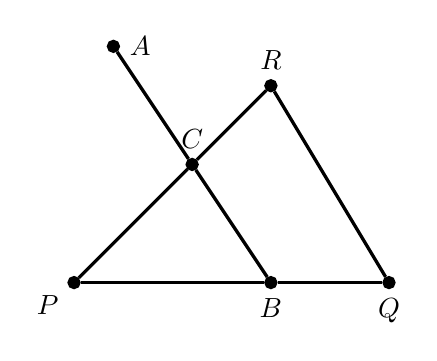
\begin{tikzpicture}
    \tikzstyle{point}=[circle,thick,draw=black,fill=black,inner sep=0pt,minimum width=4pt,minimum height=4pt]
    \node (P)[point,label={[label distance=0cm]210:$P$}] at (0,0) {};
    \node (B)[point,label={[label distance=0cm]-90:$B$}] at (2.5,0) {};
    \node (Q)[point,label={[label distance=0cm]-90:$Q$}] at (4,0) {};
    \node (C)[point,label={[label distance=0cm]90:$C$}] at (1.5,1.5) {};
    \node (R)[point,label={[label distance=0cm]90:$R$}] at (2.5,2.5) {};

    \node (A)[point,label={[label distance=0cm]0:$A$}] at (0.5,3) {};

    \draw[very thick] (P) edge node  {} (B);
    \draw[very thick] (B) edge node  {} (Q);
    \draw[very thick] (P) edge node  {} (C);
    \draw[very thick] (C) edge node  {} (R);

    \draw[very thick] (B) edge node  {} (C);
    \draw[very thick] (C) edge node  {} (A);

    \draw[very thick] (Q) edge node  {} (R);
\end{tikzpicture}
\end{document}

                \caption{$P, Q, R$ sind Fixpunkte, $B \in \overline{PQ} \setminus \Set{P,Q}$, $A \notin PQ \cup PR \cup QR$}
                \label{fig:geometry-1}
            \end{figure}

            Ist $R \notin AB$, so ist $AB \cap \overline{PR} \neq \emptyset$
            oder $AB \in \overline{RQ} \neq \emptyset$ nach \cref{satz:pasch}.
            Der Schnittpunkt $C$ ist dann Fixpunkt von $\varphi'$
            nach \cref{kor:beh2'} $\Rightarrow \varphi(A) = A$.
        \end{beweis}

        \begin{beweis}[von Beh. 1]
            Sei $R \in X \setminus PQ$. Von den drei Punkten 
            $\varphi_1(R), \varphi_2(R), \varphi_3(R)$ liegen zwei
            in der selben Halbebene bzgl. $P'Q' = \varphi_i(PQ)$.

            \Obda seien $\varphi_1(R)$ und $\varphi_2(R)$ in der 
            selben Halbebene.

            Es gilt: 
            \begin{align}
                d(P', \varphi_1(R)) &= d(\varphi_1(P), \varphi_1(R))\\
                    &= d(P, R)\\
                    &= d(\varphi_2(P), \varphi_2(R))\\
                    &= d(P', \varphi_2(R))\\
                    &= d(Q', \varphi_2(R))
            \end{align}
            und analog $d(Q', \varphi_1(R)) = d(Q', \varphi_2(R))$
        \end{beweis}
    \end{beweis}
\end{beweis}

\begin{bemerkung}
    Mit \ref{kor:14.6} lassen sich die Kongruenzsätze für Dreiecke,
    wie man sie aus der Schule kennt, beweisen.
\end{bemerkung}

\begin{proposition}\label{prop:14.7}%In Vorlesung: Proposition 14.7
    Sei $(X, d, G)$ eine Geometrie mit den Axiomen \ref{axiom:1}~-~\ref{axiom:4}.

    Dann gibt es zu jedem $g \in G$ und jedem $P \in X \setminus g$ ein
    $h \in G$ mit $P \in h$ und $g \cap h \neq \emptyset$.
\end{proposition}

\begin{figure}[htp]
    \centering
    \documentclass[varwidth=true, border=2pt]{standalone}
\usepackage{tkz-euclide}

\begin{document}
\usetkzobj{all}
\begin{tikzpicture}
    \tkzSetUpPoint[shape=circle,size=10,color=black,fill=black]
    \tkzSetUpLine[line width=1]
    \tkzDefPoints{0/0/Q, 4/1/H1, 1/2/P}
    \tkzDefPoint(1.5,3){Phelper}
    \tkzMarkAngle[arc=l,size=1cm,color=green,fill=green!20](H1,Q,P)
    \tkzDrawLine(Q,H1)

    \tkzLabelPoint[above left](Q){$Q$}
    \tkzDefLine[parallel=through P](Q,H1) \tkzGetPoint{b}
    \tkzMarkAngle[arc=l,size=1cm,color=green,fill=green!20](b,P,Phelper)
    \tkzDrawLine[dashed](P,b)
    \tkzLabelLine[pos=0.8,below](P,b){$h$}
    \tkzLabelLine[pos=-0.6,left](P,Q){$f$}
    \tkzLabelLine[pos=0.8,below](Q,H1){$g$}
    \tkzLabelPoint[above left](P){$P$}
    \tkzDrawLine[add=0.2 and 0.7](Q,P)
    \tkzDrawPoints(P,Q)
    \tkzMarkSegments[mark=||](Q,H1 P,b)
\end{tikzpicture}
\end{document}

    \caption{Situation aus \cref{prop:14.7}}
    \label{fig:bild-6}
\end{figure}

\begin{beweis}
    Sei $f \in G$ mit $P \in f$. Ist $f \cap g = \emptyset$, so setze
    $h := f$. Andernfalls sei $\Set{Q} : = f \cap g$.

    Sei $\varphi$ die eindeutige Isometrie mit $\varphi(Q) = P$,
    $\varphi(P) = P'$, die die Halbebenen bzgl. $f$ nicht vertauscht.
    
    Setze $h := \varphi(g)$.

    \underline{Z.~Z.:} $h \cap g = \emptyset$.

    Andernfalls sei $\Set{R} = h \cap g$.
\end{beweis}

\begin{bemerkung}
    Jeder Innenwinkel eines Dreiecks ist kleiner als alle nicht-anliegenden
    Außenwinkel.
\end{bemerkung}

%%%%%%%%%%%%%%%%%%%%%%%%%%%%%%%%%%%%%%%%%%%%%%%%%%%%%%%%%%%%%%%%%%%%%
% Mitschrieb vom 16.01.2014                                         %
%%%%%%%%%%%%%%%%%%%%%%%%%%%%%%%%%%%%%%%%%%%%%%%%%%%%%%%%%%%%%%%%%%%%%
\begin{beweis}
    Sei $\varphi$ die Isometrie, die $Q$ auf $P$ und $P$ auf $P'$
    mit $P' \in f, d(P,P') = d(P, Q)$ abbildet und die Halbebenen
    bzgl. $f$ erhält.
\end{beweis}

\begin{behauptung}[Herz]\label{beh:herz}
    $\varphi(g) \cap g = \emptyset$
\end{behauptung}

\begin{beweis}
    Ist $\varphi(g) \cap g \neq \emptyset$, so ist $R$ der Schnittpunkt.
\end{beweis}

\begin{figure}[htp]
    \centering
    \documentclass[varwidth=true, border=2pt]{standalone}
\usepackage{tkz-euclide}

\begin{document}
\usetkzobj{all}
\begin{tikzpicture}
    \tkzSetUpPoint[shape=circle,size=10,color=black,fill=black]
    \tkzSetUpLine[line width=1]
    \tkzDefPoints{0/0/Q, 2/0/P, 1/2/R}


    \pgfmathsetmacro{\firstAngle}{0}
    \pgfmathsetmacro{\secondAngle}{-120}
    \path[draw,red, fill=red!40] (Q) -- ++(\firstAngle:.4) arc[start angle=\firstAngle, delta angle=\secondAngle,radius=.4];

    \tkzMarkAngle[arc=l,size=0.8cm,color=green,fill=green!20](Q,R,P)
    \path[draw] ++(-50:.2) node[rotate=-50] {$\alpha$};
    \node at (1,1.5) {$\beta$};
    \tkzDrawLine(Q,P)
    \tkzDrawLine(Q,R)
    \tkzDrawLine(P,R)
    \tkzDrawPoints(P,Q,R)
    \tkzLabelPoint[below left](P){$P$}
    \tkzLabelPoint[above left](Q){$Q$}
    \tkzLabelPoint[above=0.2cm](R){$R$}
\end{tikzpicture}
\end{document}

    \caption{Skizze zu \cref{beh:herz}}
    \label{fig:bild-6}
\end{figure}

\begin{definition}\label{def:14.8}%In Vorlesung: 14.8
    \begin{defenum}
        \item \label{def:14.8a} Ein \textbf{Winkel}\xindex{Winkel} ist ein Punkt $P \in X$ 
              zusammen mit $2$ Halbgeraden mit Anfangspunkt $P$.\\
              Man schreibt: $\angle R_1 P R_2$ bzw. $\angle R_2 P R_1$\footnote{Für dieses Skript gilt: $\angle R_1 P R_2 = \angle R_2 P R_1$. Also sind insbesondere alle Winkel $ \leq 180^\circ$.}
        \item Zwei Winkel sind \textbf{gleich}, wenn es eine Isometrie gibt, 
              die den einen Winkel auf den anderen abbildet.
        \item \label{def:14.8c} $\angle R_1' P' R_2'$ heißt \textbf{kleiner} als
              $\angle R_1 P R_2$, wenn es eine Isometrie $\varphi$
              gibt, mit $\varphi(P) = P'$, $\varphi(PR'_1+) = P' R_1 +$
              und $\varphi(R_2')$ liegt in der gleichen Halbebene 
              bzgl. $PR_1$ wie $R_2$ und in der gleichen Halbebene
              bzgl. $PR_2$ wie $R_1$
        \item \label{def:14.8d} Im Dreieck $\triangle PQR$ gibt es Innenwinkel und
              Außenwinkel.
    \end{defenum}
\end{definition}

\begin{figure}[ht]
    \centering
    \subfloat[$\angle R_1' P' R_2'$ ist kleiner als $\angle R_1 P R_2$, vgl. \cref{def:14.8c}]{
        \documentclass[varwidth=true, border=2pt]{standalone}
\usepackage{tkz-euclide}
\usetkzobj{all}

\begin{document}
\begin{tikzpicture}
    \tkzSetUpPoint[shape=circle,size=10,color=black,fill=black]
    \tkzSetUpLine[line width=1]
    \tkzDefPoints{0/0/P, 1.5/0/R1S, 3/0/R1, 1/1/G, 1/2/R2}

    \tkzMarkAngle[arc=lll,size=1.2cm,color=red,fill=red!20](R1S,P,R2)
    \tkzDrawLine[add=0 and 0.3,color=green](P,R1)
    \tkzDrawLine[add=0 and 0.6](P,R2)
    \tkzLabelPoint[below left](P){$P$}
    \tkzLabelPoint[below](R1S){$R_1'$}
    \tkzLabelPoint[below](R1){$R_1$}

    \tkzInterLC(P,R1)(R1S,P) \tkzGetPoints{D}{E}
    \tkzInterLC(P,G)(R1S,P) \tkzGetPoints{F}{R2S}
    %\tkzDrawCircle(R1S,D)
    \tkzLabelPoint[below](R2S){$R_2'$}
    \tkzLabelPoint[above left](R2){$R_2$}
    \tkzDrawLine[add=0 and 1,color=green](P,R2S)
    \tkzMarkAngle[arc=l,size=0.8cm,color=green,fill=green!20](R1S,P,R2S)
    \tkzDrawPoints(P, R1S, R1, R2,R2S)
\end{tikzpicture}
\end{document}

        \label{fig:def.14.8.1}
    }%
    \subfloat[{\color{green} Innenwinkel} und {\color{blue} Außenwinkel} in $\triangle PQR$, vgl. \cref{def:14.8d}]{
        \documentclass[varwidth=true, border=2pt]{standalone}
\usepackage{tkz-euclide}
\usetkzobj{all}

\begin{document}
\begin{tikzpicture}
    \tkzSetUpPoint[shape=circle,size=10,color=black,fill=black]
    \tkzSetUpLine[line width=1]
    \tkzDefPoints{0/1/P, -1/-1/Q, 1/-1/R, -2/-1/links, 2/-1/rechts, -1.5/-2/helperLeft, 1.5/-2/helperRight, -0.25/1.5/helperTopLeft, 0.25/1.5/helperTopRight}

    \tkzMarkAngle[arc=l,size=0.6cm,color=green,fill=green!20](R,Q,P)
    \tkzMarkAngle[arc=l,size=0.6cm,color=green,fill=green!20](P,R,Q)
    \tkzMarkAngle[arc=l,size=0.6cm,color=green,fill=green!20](Q,P,R)
    \tkzMarkAngle[arc=lll,size=0.6cm,color=blue,fill=blue!20](P,Q,links)
    \tkzMarkAngle[arc=lll,size=0.6cm,color=blue,fill=blue!20](helperLeft,Q,R)
    \tkzMarkAngle[arc=lll,size=0.6cm,color=blue,fill=blue!20](helperTopLeft,P,Q)
    \tkzMarkAngle[arc=lll,size=0.6cm,color=blue,fill=blue!20](R,P,helperTopRight)
    \tkzMarkAngle[arc=lll,size=0.6cm,color=blue,fill=blue!20](rechts,R,P)
    \tkzMarkAngle[arc=lll,size=0.6cm,color=blue,fill=blue!20](Q,R,helperRight)
    \tkzDrawLine[add=0.35 and 0.35](P,Q)
    \tkzDrawLine[add=0.35 and 0.35](P,R)
    \tkzDrawLine[add=0.4 and 0.4](Q,R)



    \node at ($(P) + (0.03,0.4)$)  {$P$};
    \node at ($(Q) + (-0.3,-0.22)$)  {$Q$};
    \node at ($(R) + ( 0.3,-0.18)$)  {$R$};
    %\tkzLabelPoint[above=0.2cm](P){$P$}
    %\tkzLabelPoint[below left](Q){$Q$}
    %\tkzLabelPoint[below right](R){$R$}
    \tkzDrawPoints(P, Q, R)
\end{tikzpicture}
\end{document}

        \label{fig:def.14.8.2}
    }
    \label{fig:def.14.8.0}
    \caption{Situation aus \cref{def:14.8}}
\end{figure}

\begin{bemerkung}\label{kor:14.9}%In Vorlesung: Bemerkung 14.9
    In einem Dreieck ist jeder Innenwinkel kleiner als jeder nicht 
    anliegende Außenwinkel.
\end{bemerkung}

\begin{figure}[htp]
    \centering
    \begin{tikzpicture}
    \tkzSetUpPoint[shape=circle,size=10,color=black,fill=black]
    \tkzSetUpLine[line width=1]
    \tkzDefPoints{-1/0/Q, 0/0/M, 0/-2/A, 0/2/P, 1/0/R, -1.2/-0.5/helper}
    \tkzFillPolygon[color = green!10](Q,M,A)
    \tkzFillPolygon[color = green!10](M,P,R)
    \tkzMarkAngle[arc=l,size=0.4cm,color=red,fill=red!20](P,R,M)
    \tkzMarkAngle[arc=lll,size=0.4cm,color=green,fill=green!20](helper,Q,M)
    %\path[draw] ++(25:.3) node[rotate=0] {$\alpha$};
    %\node at (1,1.5) {$\beta$};
    \tkzDrawSegments(Q,A)
    \tkzDrawLines(Q,R A,P Q,P P,R)
    \tkzDrawPoints(Q,M,A,P,R)
    \tkzLabelPoint[below left](Q){$Q$}
    \tkzLabelPoint[below right](M){$M$}
    \tkzLabelPoint[above left](A){$A$}
    \tkzLabelPoint[above right](P){$P$}
    \tkzLabelPoint[above right](R){$R$}
\end{tikzpicture}

    \caption{Situation aus \cref{kor:14.9}}
    \label{fig:bem.14.9}
\end{figure}

\begin{beweis}
    Zeige $\angle PRQ < \angle RQP'$.

    Sei $M$ der Mittelpunkt der Strecke $\overline{QR}$. Sei
    $A \in MP^-$ mit $d(P,M) = d(M,A)$.

    Es gilt: $d(Q,M) = d(M,R)$ und $d(P,M) = d(M,A)$ sowie 
    $\angle PMR = \angle AMQ \Rightarrow \triangle MRQ$ ist
    kongruent zu $\triangle AMQ$, denn eine der beiden Isometrien, die
    $\angle PMR$ auf $\angle AMQ$ abbildet, bildet $R$ auf $Q$ und
    $P$ auf $A$ ab.

    $\Rightarrow \angle MQA = \angle MRP = \angle QRP = \angle PRQ$.

    Noch zu zeigen: $\angle MQA < \angle RQP'$, denn $A$ liegt in der
    selben Halbebene bzgl. $PQ$ wie $M$.
\end{beweis}

\begin{beweis}[von \cref{prop:14.7}]
    Wäre $\varphi(g)$ nicht parallel zu $g$, so gäbe es einen 
    Schnittpunkt $R$. Dann ist $\angle QPR < \angle RQP^-$ nach
    \cref{kor:14.9} und $\angle QPR = \angle RQP^-$, weil
    $\varphi(\angle RQP') = \angle RPQ$
\end{beweis}

\begin{folgerung}\label{folgerung:14.10}%In Vorlesung: Folgerung 14.10
    Die Summe zweier Innenwinkel in einem Dreieck ist kleiner als
    $\pi$, d.~h. es gibt eine Isometrie $\varphi$ mit $\varphi(Q) = P$
    und $\varphi(QP^+) = PR^+$, sodass $\varphi(R)$ in der gleichen
    Halbebene bzgl. $PQ$ liegt wie $R$.
\end{folgerung}

\begin{beweis}
    Die Summe eines Innenwinkels mit den anliegenden Außenwinkeln ist
    $\pi$, d.~h. die beiden Halbgeraden bilden eine Gerade.
\end{beweis}

\begin{figure}[htp]
    \centering
    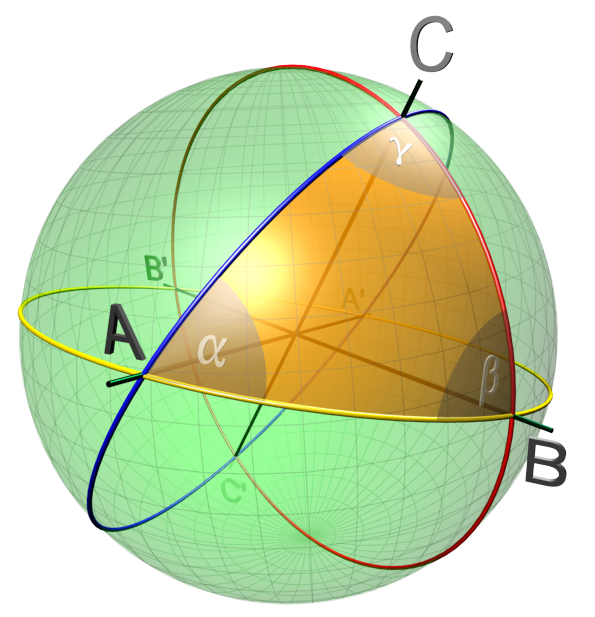
\includegraphics[width=0.4\linewidth, keepaspectratio]{figures/Spherical_triangle_3d_opti.png} 
    \caption{In der sphärischen Geometrie gibt es, im Gegensatz zur euklidischen Geometrie, Dreiecke mit drei $90^\circ$-Winkeln.}
    \label{fig:bem.14.9}
\end{figure}

\begin{proposition}\label{prop:14.11}%In Vorlesung: Proposition 14.11
    In einer Geometrie mit den Axiomen \ref{axiom:1}~-~\ref{axiom:4}
    ist in jedem Dreieck die Summe der Innenwinkel $\leq \pi$.
\end{proposition}

Sei im Folgenden \enquote{IWS} die \enquote{Innenwinkelsumme}.

\begin{beweis}
    Sei $\triangle$ ein Dreieck mit $\IWS(\triangle) = \pi + \varepsilon$

    \begin{figure}[ht]
        \centering
        \subfloat[Summe der Winkel $\alpha$, $\beta$ und $\gamma$]{
            \resizebox{0.4\linewidth}{!}{\begin{tikzpicture}
    \tkzSetUpPoint[shape=circle,size=10,color=black,fill=black]
    \tkzSetUpLine[line width=1]
    \tkzDefPoints{0/0/P, 1/0/helperRight, 1/1/helperTopRight, -1/1/helperTopLeft, -1/0/helperLeft, -1/-0.3/helperBottomLeft}

    \tkzMarkAngle[arc=l,size=0.8cm,color=green,fill=green!20](helperRight,P,helperTopRight)
    \tkzMarkAngle[arc=ll,size=0.8cm,color=blue,fill=blue!20](helperTopRight,P,helperTopLeft)
    \tkzMarkAngle[arc=lll,size=0.8cm,color=red,fill=red!20](helperTopLeft,P,helperBottomLeft)
    \path[draw] ++(25:.4) node[rotate=0] {$\alpha$};
    \path[draw] ++(90:.4) node[rotate=0] {$\beta$};
    \path[draw] ++(160:.4) node[rotate=0] {$\gamma$};

    \tkzDrawLine[add=0 and 1.0](P, helperRight)
    \tkzDrawLine[add=0 and 0.3](P, helperTopRight)
    \tkzDrawLine[add=0 and 0.3](P, helperTopLeft)
    \tkzDrawLine[add=0 and 1.0](P, helperLeft)
    \tkzDrawLine[add=0 and 0.8](P, helperBottomLeft)

    \tkzDrawPoints(P)
    \tkzLabelPoint[below](P){$P$}
\end{tikzpicture}
}
            \label{fig:prop14.11.1}
        }%
        \subfloat[Situation aus \cref{prop:14.11}]{
            \resizebox{0.4\linewidth}{!}{\documentclass[varwidth=true, border=2pt]{standalone}
\usepackage{tkz-euclide}

\begin{document}
\usetkzobj{all}
\begin{tikzpicture}
    \tkzSetUpPoint[shape=circle,size=10,color=black,fill=black]
    \tkzSetUpLine[line width=1]
    \tkzDefPoints{0/0/A, 4/0/B, 2/2/C, 6/2/D}

    \tkzMarkAngle[arc=l,size=0.8cm,color=green,fill=green!20](B,A,C)
    \path[draw] ++(25:.3) node[rotate=0] {$\alpha$};
    \node at (1,1.5) {$\beta$};
    \tkzDrawSegments(A,B A,C A,D B,C C,D)
    \tkzDrawPoints(A,B,C,D)
    \tkzLabelPoint[below left](A){$A$}
    \tkzLabelPoint[below right](B){$B$}
    \tkzLabelPoint[above left](C){$C$}
    \tkzLabelPoint[above right](D){$D$}
\end{tikzpicture}
\end{document}
}
            \label{fig:prop14.11.2}
        }
        \label{fig:prop14.11.0}
        \caption{Situation aus \cref{prop:14.11}}
    \end{figure}

    Sei $\alpha$ ein Innenwinkel von $\triangle$.

    \begin{behauptung}
        Es gibt ein Dreieck $\triangle'$ mit 
        $\IWS(\triangle') = \IWS(\triangle)$ und einem Innenwinkel
        $\alpha' \leq \frac{\alpha}{2}$.

        Dann gibt es für jedes $n$ ein $\triangle_n$ mit $\IWS(\triangle_n) = \IWS(\triangle)$
        und Innenwinkel $\alpha' \leq \frac{\alpha}{2^n}$. Für $\frac{\alpha}{2^n} < \varepsilon$
        ist dann die Summe der beiden Innenwinkel
        um $\triangle_n$ größer als $\pi \Rightarrow$ Widerspruch zu
        \cref{folgerung:14.10}.
    \end{behauptung}

    \begin{beweis}[der Behauptung]
        Sei $M$ der Mittelpunkt $\overline{RC}$ und $A' \in MA^-$ mit
        $d(A', M) = d(A, M) \Rightarrow \triangle(MA'C)$ und
        $\triangle(MAB)$ sind kongruent.
        $\Rightarrow \angle ABM = \angle A'CM$ und $\angle MA'C = \angle MAB$.
        $\Rightarrow \alpha + \beta + \gamma =\IWS(\triangle ABC) = \IWS(\triangle AA'C)$
        und $\alpha_1 + \alpha_2 = \alpha$, also \obda $\alpha_1 \leq \frac{\alpha}{2}$
    \end{beweis}
\end{beweis}
%%%%%%%%%%%%%%%%%%%%%%%%%%%%%%%%%%%%%%%%%%%%%%%%%%%%%%%%%%%%%%%%%%%%%
% Mitschrieb vom 21.01.2014                                         %
%%%%%%%%%%%%%%%%%%%%%%%%%%%%%%%%%%%%%%%%%%%%%%%%%%%%%%%%%%%%%%%%%%%%%
\begin{bemerkung}\label{bem:14.12}%In Vorlesung: Bemerkung 14.12
    In einer euklidischen Ebene ist in jedem Dreieck die Innenwinkelsumme
    gleich $\pi$.
\end{bemerkung}

\begin{figure}[htp]
    \centering
    \begin{tikzpicture}
    \tkzSetUpPoint[shape=circle,size=10,color=black,fill=black]
    \tkzSetUpLine[line width=1]
    \tkzDefPoints{0/0/A, 3/0/B, 2/2/C}
    \tkzDefPoints{0/2/Phelper, 1.75/2.5/PaboveLeft, 2.5/2.5/PaboveRight}
    \tkzMarkAngle[arc=l,size=0.7cm,color=red,fill=red!20](B,A,C)
    \tkzMarkAngle[arc=ll,size=0.7cm,color=orange,fill=orange!20](C,B,A)
    \tkzMarkAngle[arc=lll,size=0.7cm,color=green,fill=green!20](A,C,B)
    \tkzMarkAngle[arc=l,size=0.7cm,color=red,fill=red!20](Phelper,C,A)
    \tkzMarkAngle[arc=ll,size=0.7cm,color=orange,fill=orange!20](PaboveLeft,C,Phelper)
    \tkzDefLine[parallel=through C](A,B) \tkzGetPoint{Phelper2}
    \tkzMarkAngle[arc=l,size=0.7cm,color=red,fill=red!20](Phelper2,C,PaboveRight)
    \tkzLabelAngle[pos=0.4](Phelper2,C,PaboveRight){$\alpha$}
    \tkzLabelAngle[pos=-0.4](Phelper,C,A){$\alpha''$}
    \tkzLabelAngle[pos=0.4](B,A,C){$\alpha$}
    \tkzLabelAngle[pos=0.4](C,B,A){$\beta$}
    \tkzLabelAngle[pos=0.4](PaboveLeft,C,Phelper){$\beta$}
    \tkzLabelAngle[pos=0.4](A,C,B){$\gamma$}
    \tkzDrawLine(A,B)
    \tkzDrawLine[add=0.2 and 0.4](A,C)
    \tkzDrawLine[add=0.2 and 0.4](B,C)

    \node at ($(A)+(-0.47,-0.2)$)  {$A$};
    \node at ($(B)+(0.35,-0.2)$)  {$B$}; % \tkzLabelPoint[below](B){$B$} is not accurate enough
    \node at ($(C)+(0.05,0.3)$)  {$C$};
    \tkzDrawLine[add=0.6 and -0.1](C, Phelper2)
    %\tkzMark[mark=||](C, PaboveRight)
    %\tkzLabelLine[pos=0.8,below](A,B){$c$}
    \tkzDrawPoints(A,B,C)
    \tkzLabelSegment[pos=0.7,below](C,Phelper2){$g$}
    \tkzMarkSegments[mark=||](A,B C,Phelper2)
\end{tikzpicture}

    \caption{Situation aus \cref{bem:14.12}}
    \label{fig:14.12}
\end{figure}

\begin{beweis}
    Sei $g$ eine Parallele von $AB$ durch $C$. 

    \begin{itemize}
        \item Es gibt $\alpha' = \alpha$ wegen \cref{prop:14.7}.
        \item Es gibt $\beta' = \beta$ wegen \cref{prop:14.7}.
        \item Es gibt $\alpha'' = \alpha'$ wegen \cref{ub11:aufg1}.
    \end{itemize}
    $\Rightarrow \IWS(\triangle ABC) = \gamma + \alpha'' + \beta' = \pi$
\end{beweis}

\section{Weitere Eigenschaften einer euklidischen Ebene}
\subsection{Strahlensatz}
\begin{satz}
    In ähnlichen Dreiecken sind Verhältnisse entsprechender Seiten gleich.
\end{satz}

\begin{figure}[htp]
    \centering
    \documentclass[varwidth=true, border=10pt]{standalone}
\usepackage{tkz-euclide}
\usepackage{tkz-fct} 
\newcommand{\iu}{{i\mkern1mu}} % imaginary unit

\begin{document}
\usetkzobj{all}
\begin{tikzpicture}
    \tkzSetUpPoint[shape=circle,size=3,color=black,fill=black]
    \tkzSetUpLine[line width=0.5]
    \tkzInit[xmax=4.5,ymax=3,xmin=-1,ymin=0]
    \tkzDefPoints{0/0/O, 3/3/lz, 2/2/z, 3/0/lzx, 2/0/zx}
    \tkzDrawLines(O,lz zx,z)
    \tkzDrawLine[add=0 and 0.2](lzx,lz)
    \tkzAxeXY[ticks=false]

    %\tkzDrawArc[R,line width=1pt,color=red](m1,1.5 cm)(0,180)
    %\tkzDrawArc[R,line width=1pt](m2,2.5 cm)(0,180)
    \tkzDrawPoints(z,lz)
    \tkzLabelPoint[left](z) {$z$}
    \tkzLabelPoint[above right](zx) {$x$}
    \tkzLabelPoint[right](lz) {$\lambda^2 z$}
    \tkzLabelPoint[above right](lzx) {$\lambda^2 x$}
    %\node[red] at ($(m1)+(1.5,-0.2)$)  {$m+1$};
\end{tikzpicture}
\end{document}

    \caption{Strahlensatz}
    \label{fig:bild-2}
\end{figure}

\begin{beweis}
    TODO
\end{beweis}

\begin{figure}[htp]
    \centering
    \documentclass[varwidth=true, border=2pt]{standalone}
\usepackage{tikz}
\usepackage{tkz-euclide}

\begin{document}
\usetkzobj{all}
\begin{tikzpicture}
    \tkzSetUpPoint[shape=circle,size=10,color=black,fill=black]
    \tkzSetUpLine[line width=1]
    \tkzDefPoints{0/0/A, 3/0/B', 2/2/C, 4/4/C'}
    \tkzDefLine[parallel=through C](B',C') \tkzGetPoint{Phelper}
    \tkzInterLL(A,B')(C,Phelper) \tkzGetPoint{B}
    \tkzDrawLine[add=0 and 0.2](A,B')
    \tkzDrawLine[add=0 and 0.2](A,C')
    \tkzDrawSegment(B',C')

    \node at ($(A)+(-0.1,-0.2)$)  {$A$};
    \node at ($(B')+(0.2,-0.2)$)  {$B'$};
    \node at ($(C')+(0,0.4)$)  {$C'$};
    \node at ($(B)+(0.2,-0.2)$)  {$B$};
    \node at ($(C)+(0.28,0.5)$)  {$C$};
    \tkzDrawPolygon[ultra thick,color=blue,fill=blue!20](A,B',C') 
    \tkzDrawPolygon[line width=0.3pt,color=red,fill=red!20](A,B,C) 
    \tkzDrawPoints(A,B',C',B,C)
    \tkzLabelSegment[below,red](A,B){$c$}
    \tkzLabelSegment[left,red](A,C){$b$}
    \tkzLabelSegment[right,red](B,C){$a$}
    \tkzLabelSegment[below,blue,pos=0.8](A,B'){$c'$}
    \tkzLabelSegment[left,blue,pos=0.8](A,C'){$b'$}
    \tkzLabelSegment[right,blue](B',C'){$a'$}
\end{tikzpicture}
\end{document}

    \caption{Die Dreiecke $\triangle ABC$ und $\triangle AB'C'$ sind ähnlich.}
    \label{fig:bild-3}
\end{figure}

\subsection{Flächeninhalt}
\begin{definition}
    \enquote{Simplizialkomplexe} in euklidischer Ebene $(X,d)$ heißen
    \textbf{flächengleich}\xindex{Simplizialkomplexe!flächengleiche},
    wenn sie sich in kongruente Dreiecke zerlegen lassen.
\end{definition}

\begin{figure}[ht]
    \centering
    \subfloat[TODO]{
        \documentclass[varwidth=true, border=2pt]{standalone}
\usepackage{tkz-euclide}

\begin{document}
\usetkzobj{all}
\begin{tikzpicture}
    \tkzSetUpPoint[shape=circle,size=10,color=black,fill=black]
    \tkzSetUpLine[line width=1]
    \tkzDefPoints{0/0/A, 4/0/B, 4/2/C, 0/2/D, 3/2/E, 4/1/F, 1/0/G, 1/-1/H}
    \tkzDrawPolygon[fill=black!20](A,B,C,D)
    \tkzDrawPolygon[orange,fill=orange!20](E,C,F)
    \tkzDrawPolygon[orange,fill=orange!20](A,G,H)
    \tkzDrawPoints(A,B,C,D)
\end{tikzpicture}
\end{document}

        \label{fig:bild-4}
    }%
    \subfloat[TODO]{
        \documentclass[varwidth=true, border=2pt]{standalone}
\usepackage{tkz-euclide}
\usepackage{tikz}
\usetikzlibrary{patterns}

\begin{document}
\usetkzobj{all}
\begin{tikzpicture}
    \tkzSetUpPoint[shape=circle,size=10,color=black,fill=black]
    \tkzSetUpLine[line width=1]
    \tkzDefPoints{0/0/A, 4/0/B, 4/2/C, 0/2/D}
    \tkzDrawPolygon(A,B,C,D)
    \tkzDrawPolygon[pattern=north east lines](A,B,C)
    \tkzDrawPolygon[pattern=north west lines](C,D,A)
    \tkzDrawPoints(A,B,C,D)
\end{tikzpicture}
\end{document}

        \label{fig:bild-5}
    }%
    \label{fig:flaechengleichheit}
    \caption{Flächengleichheit}
\end{figure}

Der Flächeninhalt eines Dreiecks ist $\nicefrac{1}{2} \cdot \text{Grundseite} \cdot \text{Höhe}$.

\begin{figure}[htp]
    \centering
    
\begin{tikzpicture}
    \path (0,0)  edge [bend angle=10,bend right] node[label=TODO] {} (-1,-1.5);
\end{tikzpicture}

    \caption{Flächenberechnung im Dreiecks}
    \label{fig:flaechenberechnung-dreieck}
\end{figure}

\underline{Zu zeigen:} Unabhängigkeit von der gewählten Grundseite.

\begin{figure}[htp]
    \centering
    \begin{tikzpicture}
    \tkzSetUpPoint[shape=circle,size=10,color=black,fill=black]
    \tkzSetUpLine[line width=1]
    \tkzDefPoints{0/0/A, 4/0/B, 3/3/C}

    \tkzDefLine[orthogonal=through A,/tikz/overlay](B,C) \tkzGetPoint{helper}
    \tkzInterLL(B,C)(A,helper) \tkzGetPoint{La}
    \tkzDefLine[orthogonal=through C,/tikz/overlay](A,B) \tkzGetPoint{helper}
    \tkzInterLL(A,B)(C,helper) \tkzGetPoint{Lc}

    \tkzInterLL(A,La)(C,Lc) \tkzGetPoint{orthocenter}

    \tkzMarkAngle[arc=l,size=1.0cm,color=red,fill=red!20](B,A,La)
    \tkzLabelAngle[pos=0.8](B,A,La){$\alpha$}

    \tkzMarkAngle[arc=l,size=1.0cm,color=red,fill=red!20](Lc,C,B)
    \tkzLabelAngle[pos=0.8](Lc,C,B){$\alpha$}

    \tkzMarkAngle[arc=ll,size=0.6cm,color=green,fill=green!20](A,orthocenter,Lc)
    \tkzLabelAngle[pos=0.4](A,orthocenter,Lc){$\gamma$}

    \tkzMarkAngle[arc=ll,size=0.4cm,color=green,fill=green!20](La,orthocenter,C)
    \tkzLabelAngle[pos=0.2](La,orthocenter,C){$\gamma$}

    \tkzDrawPolygon(A,B,C)

    \node at ($(A)+(-0.47,-0.2)$){$A$};
    \node at ($(B)+(0.35,-0.2)$) {$B$}; % \tkzLabelPoint[below](B){$B$} is not accurate enough
    \node at ($(C)+(0.05,0.3)$)  {$C$};
    \node at ($(La)+(0.25,0.1)$)  {$L_A$};
    \node at ($(Lc)+(0,-0.25)$)  {$L_C$};

    \tkzDrawSegment(C,Lc)
    \tkzDrawSegments(A,La)
    \tkzDrawPolygon[pattern=north east lines](A,B,La)
    \tkzDrawPolygon[pattern=north west lines](Lc,B,C)
    \tkzDrawPoints(A,B,C,La,Lc)
    %\tkzLabelSegment[pos=0.7,below](A,B){$c$}
\end{tikzpicture}

    \caption{$\triangle ABL_a$ und $\triangle C{L_C}B$ sind ähnlich, weil $\IWS = \pi$}
    \label{fig:flaechenberechnung-dreieck-2}
\end{figure}

$\overset{\text{Strahlensatz}}{\Rightarrow} \frac{a}{h_c} = \frac{c}{h_a} \rightarrow a \cdot h_a = c \cdot h_c$

\begin{satz}[Satz des Pythagoras]
    Im rechtwinkligen Dreieck gilt $a^2 + b^2 = c^2$, wobei $c$ die
    Hypothenuse und $a, b$ die beiden Katheten sind.
\end{satz}

\begin{figure}[ht]
    \centering
    \subfloat[$a,b$ sind Katheten und $c$ ist die Hypothenuse]{
        \begin{tikzpicture}
    \tkzSetUpPoint[shape=circle,size=10,color=black,fill=black]
    \tkzSetUpLine[line width=1]
    \tkzDefPoints{0/0/A, 5/0/B}
    \tkzInterCC[R,/tikz/overlay](A,4cm)(B,3cm) \tkzGetPoints{C}{D}
    \tkzDrawPolygon(A,B,C)
    \tkzDrawPoints(A,B,C)
    \tkzLabelSegment[below](A,B){$c$}
    \tkzLabelSegment[above left](A,C){$b$}
    \tkzLabelSegment[above right](B,C){$a$}
    \tkzLabelPoint[below](A){$A$}
    \tkzLabelPoint[below](B){$B$}
    \tkzLabelPoint[above](C){$C$}
    \tkzLabelAngle[pos=0.24](A,C,B){$\cdot$}
    \tkzMarkAngle[arc=l,size=0.4cm](A,C,B)
\end{tikzpicture}

        \label{fig:pythagoras-bezeichnungen}
    }%
    \subfloat[Beweisskizze]{
        \documentclass[varwidth=true, border=2pt]{standalone}
\usepackage{tkz-euclide}

\begin{document}
\usetkzobj{all}
\begin{tikzpicture}
    \tkzSetUpPoint[shape=circle,size=10,color=black,fill=black]
    \tkzSetUpLine[line width=1]
    \tkzDefPoints{0/0/A, 4/0/B, 4/4/C, 0/4/D, 1/0/W, 4/1/X, 3/4/Y, 0/3/Z}
    \tkzDrawPolygon(A,B,C,D)
    \tkzDrawPolygon(W,X,Y,Z)
    \tkzLabelSegment[below](A,W){$b$}
    \tkzLabelSegment[below](W,B){$a$}
    \tkzLabelSegment[right](B,X){$b$}
    \tkzLabelSegment[right](X,C){$a$}
    \tkzLabelSegment[above](C,Y){$b$}
    \tkzLabelSegment[above](Y,D){$a$}
    \tkzLabelSegment[left](D,Z){$b$}
    \tkzLabelSegment[left](Z,A){$a$}
    \tkzLabelAngle[pos=-0.24](D,C,B){$\cdot$}
    \tkzMarkAngle[arc=l,size=0.4cm](D,C,B)
    \tkzLabelAngle[pos=0.24](C,B,A){$\cdot$}
    \tkzMarkAngle[arc=l,size=0.4cm](C,B,A)
    \tkzLabelAngle[pos=0.24](B,A,D){$\cdot$}
    \tkzMarkAngle[arc=l,size=0.4cm](B,A,D)
    \tkzLabelAngle[pos=0.24](A,D,C){$\cdot$}
    \tkzMarkAngle[arc=l,size=0.4cm](A,D,C)
    \tkzLabelAngle[pos=0.24](W,Z,Y){$\gamma$}
    \tkzMarkAngle[arc=l,size=0.4cm](W,Z,Y)
\end{tikzpicture}
\end{document}

        \label{fig:bild-5}
    }%
    \label{fig:flaechengleichheit}
    \caption{Satz des Pythagoras}
\end{figure}

\begin{beweis}
    $(a+b) \cdot (a+b) = a^2 + 2ab + b^2 = c^2 +4 \cdot (\frac{1}{2} \cdot a \cdot b)$
\end{beweis}

\begin{satz}\label{satz:14.13} %In Vorlesung: Satz 14.13
    Bis auf Isometrie gibt es genau eine euklidische Ebene, nämlich
    $X=\mdr^2$, $d = \text{euklidischer Abstand}$, $G = \text{Menge der üblichen Geraden}$.
\end{satz}

\begin{beweis}\leavevmode
    \begin{enumerate}[label=(\roman*)]
        \item $(\mdr^2, d_\text{Euklid})$ ist offensichtlich eine euklidische Ebene.
        \item Sei $(X,d)$ eine euklidische Ebene und $g_1, g_2$ Geraden
              in $X$, die sich in einem Punkt $0$ im rechten Winkel
              schneiden. Sei $X$ der Fußpunkt des Lots von $P$ auf
              $g_1$ (vgl. \cref{ub11:aufg3.c}).

              Sei $Y$ der Fußpunkt des Lots von $P$ auf $g_2$.

              Setze $h(P) := (x_P, y_P)$ mit 
              $x_P := d(X, 0)$ und $y_P := d(Y, 0)$.

            \begin{figure}[ht]
                \centering
                \subfloat[Schritt 1]{
                    \resizebox{0.45\linewidth}{!}{\documentclass[varwidth=true, border=2pt]{standalone}
\usepackage{tkz-euclide}
\usepackage{tikz}
\usetikzlibrary{patterns}

\begin{document}
\usetkzobj{all}
\begin{tikzpicture}
    \tkzSetUpPoint[shape=circle,size=10,color=black,fill=black]
    \tkzSetUpLine[line width=1]
    \tkzDefPoints{0/0/O, 1/0/X, 0/1/Y, 2/1/P}
    \tkzDrawLine[add=3 and 2](O,X)
    \tkzLabelLine[below,pos=3](O,X){$g_1$}
    \tkzLabelLine[right,pos=3](O,Y){$g_2$}
    \tkzDrawLine[add=3 and 2](O,Y)

    \tkzLabelPoint(P){$P$}
    \node at ($(-2,2)$){$X$};
    \tkzDrawPoints(P)
\end{tikzpicture}
\end{document}
}
                    \label{fig:14.13.1}
                }%
                \subfloat[Schritt 2]{
                    \resizebox{0.45\linewidth}{!}{\begin{tikzpicture}
    \tkzSetUpPoint[shape=circle,size=10,color=black,fill=black]
    \tkzSetUpLine[line width=1]
    \tkzDefPoints{0/0/O, 1/0/X, 0/1/Y, 2/1/P}

    \tkzMarkAngle[fill=green!20,size=0.3cm,opacity=.5](X,O,Y)
    \tkzLabelAngle[pos=0.15](X,O,Y){$\cdot$}

    \tkzDrawLine[add=3 and 2](O,X)
    \tkzLabelLine[below,pos=3](O,X){$g_1$}
    \tkzLabelLine[right,pos=3](O,Y){$g_2$}
    \tkzDrawLine[add=3 and 2](O,Y)

    \tkzDefLine[orthogonal=through P,/tikz/overlay](O,X) \tkzGetPoint{helper}
    \tkzInterLL(O,X)(P,helper) \tkzGetPoint{xp}
    \draw [decorate,decoration={brace,amplitude=4pt,mirror}]
        (O) -- (xp) node [black,midway,xshift=0cm, yshift=-0.3cm] 
        {\footnotesize $x_P$};

    \tkzDefLine[orthogonal=through P,/tikz/overlay](O,Y) \tkzGetPoint{helper}
    \tkzInterLL(O,Y)(P,helper) \tkzGetPoint{yp}
    \draw [decorate,decoration={brace,amplitude=4pt}]
        (O) -- (yp) node [black,midway,xshift=-0.4cm] 
        {\footnotesize $y_P$};

    \tkzDrawPolygon(O,xp,P,yp)

    \tkzLabelPoint[above right](P){$P$}
    \tkzLabelPoint[below left](O){$0$}
    \tkzLabelPoint[below](xp){$P_X$}
    \tkzLabelPoint[left](Y){$P_Y$}
    \node at ($(-2,2)$){$X$};
    \tkzDrawPoints(P,Y,xp)
\end{tikzpicture}}
                    \label{fig:14.13.2}
                }%
                \label{fig:14.13.0.1}
                \caption{Beweis zu \cref{satz:14.13}}
            \end{figure}

            Dadurch wird $h:X \rightarrow \mdr^2$ auf dem Quadranten
            definiert, in dem $P$ liegt (d.~h. $\forall Q \in X \text{ mit } \overline{PQ} \cap g_1 = \emptyset = \overline{PQ} \cap g_2$)
            Fortsetzung auf ganz $X$ durch konsistente Vorzeichenwahl.

            \begin{behauptung}[1]
                $h$ ist surjektiv
            \end{behauptung}
            \begin{behauptung}[2]
                $h$ ist abstandserhaltend ($\rightarrow$ injektiv)
            \end{behauptung}
            \begin{beweis}[von 1]
                Sei $(x, y) \in \mdr^2$, z.~B. $x \geq 0, y \geq 0$.
                Sei $P' \in g_1$ mit $d(0, P') = x$ und
                $P'$ auf der gleichen Seite von $g_2$ wie $P$.
            \end{beweis}
            \begin{beweis}[von 2]
                \begin{figure}[ht]
                    \centering
                    \subfloat[Schritt 1]{
                        \resizebox{0.45\linewidth}{!}{\begin{tikzpicture}
    \tkzSetUpPoint[shape=circle,size=10,color=black,fill=black]
    \tkzSetUpLine[line width=1]
    \tkzDefPoints{0/0/O, 1/0/X, 0/1/Y, 2/1/P}

    \tkzMarkAngle[fill=green!20,size=0.3cm,opacity=.5](X,O,Y)
    \tkzLabelAngle[pos=0.15](X,O,Y){$\cdot$}

    \tkzDrawLine[add=3 and 2](O,X)
    \tkzLabelLine[below,pos=3](O,X){$g_1$}
    \tkzLabelLine[right,pos=3](O,Y){$g_2$}
    \tkzDrawLine[add=3 and 2](O,Y)

    \tkzDefLine[orthogonal=through P,/tikz/overlay](O,X) \tkzGetPoint{helper}
    \tkzInterLL(O,X)(P,helper) \tkzGetPoint{xp}
    \draw [decorate,decoration={brace,amplitude=4pt,mirror}]
        (O) -- (xp) node [black,midway,xshift=0cm, yshift=-0.3cm] 
        {\footnotesize $x_P$};

    \tkzDefLine[orthogonal=through P,/tikz/overlay](O,Y) \tkzGetPoint{helper}
    \tkzInterLL(O,Y)(P,helper) \tkzGetPoint{yp}
    \draw [decorate,decoration={brace,amplitude=4pt}]
        (O) -- (yp) node [black,midway,xshift=-0.4cm] 
        {\footnotesize $y_P$};

    \tkzDrawPolygon(O,xp,P,yp)

    \tkzLabelPoint[above right](P){$P$}
    \tkzLabelPoint[below left](O){$0$}
    \tkzLabelPoint[below](xp){$P_X$}
    \tkzLabelPoint[left](Y){$P_Y$}
    \node at ($(-2,2)$){$X$};
    \tkzDrawPoints(P,Y,xp)
\end{tikzpicture}}
                        \label{fig:14.13.3}
                    }%
                    \subfloat[Schritt 2 (Bild 13)]{
                        \resizebox{0.45\linewidth}{!}{
\begin{tikzpicture}
    \path (0,0)  edge [bend angle=10,bend right] node[label=TODO] {} (-1,-1.5);
\end{tikzpicture}
}
                        \label{fig:14.13.4}
                    }%
                    \label{fig:14.13.0.2}
                    \caption{Beweis zu \cref{satz:14.13}}
                \end{figure}
                Zu Zeigen: $d(P, Q) = d(h(P), h(Q))$

                $d(P, Q)^2 \overset{\text{Pythagoras}}{=} d(P, R)^2 + d(R, Q)^2 = (y_Q - y_P)^2 + (x_Q - x_P)^2$.

                $h(Q) = (x_Q, y_Q)$
            \end{beweis}
    \end{enumerate}
\end{beweis}
%%%%%%%%%%%%%%%%%%%%%%%%%%%%%%%%%%%%%%%%%%%%%%%%%%%%%%%%%%%%%%%%%%%%%
% Mitschrieb vom 23.01.2014                                         %
%%%%%%%%%%%%%%%%%%%%%%%%%%%%%%%%%%%%%%%%%%%%%%%%%%%%%%%%%%%%%%%%%%%%%
\section{Hyperbolische Geometrie}
\begin{definition}
    Sei
        \[\mdh:= \Set{z \in \mdc | \Im(z) > 0} = \Set{(x,y) \in \mdr^2 | y > 0}\]
    die obere Halbebene bzw. Poincaré-Halbebene und $G = G_1 \cup G_2$
    mit
        \begin{align*}
            G_1 &= \Set{g_1 \subseteq \mdh | \exists m \in \mdr, r \in \mdr_{>0}: g_1 = \Set{z \in \mdc : |z-m|=r}}\\
            G_2 &= \Set{g_2 \subseteq \mdh | \exists x \in \mdr: g_2 = \Set{z \in \mdc: \Re(z) = x} \cap \mdh}
        \end{align*}

    Die Elemente von $\mdh$ heißen \textbf{hyperbolische Geraden}\xindex{Gerade!hyperbolische}
\end{definition}

\begin{bemerkung}[Eigenschaften der hyperbolischen Geraden]
    Die hyperbolischen Geraden erfüllen\dots
    \begin{bemenum}
        \item \dots die Inzidenzaxiome \ref{axiom:1}
        \item \dots das Anordnungsaxiom \ref{axiom:3.2}
        \item \dots nicht das Parallelenaxiom \ref{axiom:5}
    \end{bemenum}
\end{bemerkung}

\begin{beweis}\leavevmode
    \begin{enumerate}[label=\alph*), ref=\theproposition (\alph*)]
        \item Offensichtlich sind \ref{axiom:1.3} und \ref{axiom:1.2}
              erfüllt. Für \ref{axiom:1.1} gilt:\\
              Gegeben $z_1, z_2 \in \mdh$\\
              \textbf{Existenz:} $\Re(z_1) = \Re(z_2)$
              $\Rightarrow z_1$ und $z_2$ liegen auf
              \[g = \Set{z \in \mdc | \Re(z) = \Re(z_1) \land \mdh}\]

            \begin{figure}[ht]
                \centering
                \subfloat[Fall 1]{
                    \resizebox{0.45\linewidth}{!}{\documentclass[varwidth=true, border=10pt]{standalone}
\usepackage{tkz-euclide}
\usepackage{tikz}
\usetikzlibrary{patterns}

\begin{document}
\usetkzobj{all}
\begin{tikzpicture}
    \tkzSetUpPoint[shape=circle,size=3,color=black,fill=black]
    \tkzSetUpLine[line width=1]
    \tkzInit[xmax=5,ymax=4,xmin=-1,ymin=0]
    \tkzDefPoints{2/2/Z1,2/3/Z2,2/0/A}
    \tkzAxeXY

    \tkzDrawLine[add=2 and 1, color=orange](Z1,Z2)
    \tkzDrawPoints(Z1, Z2)
    \tkzLabelPoint[right](Z1){$Z_1$}
    \tkzLabelPoint[right](Z2){$Z_2$}
    \node[orange] at ($(A)+(0.5,0.3)$)  {$\Re(Z_1)$};
\end{tikzpicture}
\end{document}
}
                    \label{fig:hyperbolische-geometrie-axiom-1-1}
                }%
                \subfloat[Fall 2]{
                    \resizebox{0.45\linewidth}{!}{\documentclass[varwidth=true, border=10pt]{standalone}
\usepackage{tkz-euclide}
\usepackage{tikz}
\usetikzlibrary{patterns}

\begin{document}
\usetkzobj{all}
\begin{tikzpicture}
    \tkzSetUpPoint[shape=circle,size=3,color=black,fill=black]
    \tkzSetUpLine[line width=1]
    \tkzInit[xmax=5,ymax=4,xmin=-1,ymin=0]
    \tkzDefPoints{1/1/Z1,2/2/Z2,3/0/A}
    \tkzAxeXY

    \tkzDrawPoints(Z1, Z2)
    \tkzLabelPoint[right](Z1){$Z_1$}
    \tkzLabelPoint[below](Z2){$Z_2$}
    \node (m) at ($(Z1)!0.5!(Z2)$) {};
    \tkzDrawSegments[dashed](Z1,Z2 A,Z1 A,Z2)

    \tkzDefLine[perpendicular=through m](Z1,Z2)\tkzGetPoint{c}
    \tkzDrawLine[add=2 and 1,dashed,thick](m, c)
    \tkzDrawArc[R,line width=1pt,color=orange](A,2.24 cm)(0,180)
\end{tikzpicture}
\end{document}
}
                    \label{fig:hyperbolische-geometrie-axiom-1-2}
                }%
                \label{fig:hyperbolische-geometrie-axiom-1-0}
                \caption{Zwei Punkte liegen in der hyperbolischen Geometrie immer auf genau einer Geraden}
            \end{figure}
        \item TODO
        \item Siehe \cref{fig:hyperbolische-halbebene-axiom-5}.
            \begin{figure}[htp]
                \centering
                \begin{tikzpicture}
    \tkzSetUpPoint[shape=circle,size=3,color=black,fill=black]
    \tkzSetUpLine[line width=1]
    \tkzInit[xmax=6,ymax=5,xmin=-5,ymin=0]
    \tkzDefPoints{-2/0/A,3.5/0/B,-0.85/0/C,2/0/D,2/2/P}
    \tkzDefPoints{-1/0/X, -1/5/Y}
    \tkzDrawLine[add=0.1 and 0.1](X,Y)
    \tkzAxeXY

    \tkzDrawArc[R,line width=1pt,color=red](A,0.5 cm)(0,180)
    \tkzDrawArc[R,line width=1pt](B,2.5 cm)(0,180)
    \tkzDrawArc[R,line width=1pt](C,3.5 cm)(0,180)
    \tkzDrawArc[R,line width=1pt](D,2.0 cm)(0,180)
    \tkzDrawPoints(P)
\end{tikzpicture}

                \caption{Hyperbolische Geraden erfüllen \ref{axiom:5} nicht.}
                \label{fig:hyperbolische-halbebene-axiom-5}
            \end{figure}
    \end{enumerate}
\end{beweis}

\begin{proposition}%In Vorlesung: Proposition 15.2
    \begin{propenum}
        \item Die Gruppe $\SL_2(\mdr)$ operiert auf $\mdh$ durch
              \[\sigma(z):= \begin{pmatrix}a & b\\c & d\end{pmatrix} \circ z := \frac{az + b}{cz + d}\]
        \item Es ist $\sigma(z) = (-\sigma)(z)$ für alle $\sigma \in \SL_2(\mdr)$
              und $z \in \mdh$. Daher operiert $\PSL_2(\mdr) = \SL_2(\mdr) /_{(\pm I)}$
              auf $\mdh$.
        \item $\PSL_2(\mdr)$ operiert auf $\mdr \cup \Set{\infty}$.
              Diese Gruppenoperation ist 3-fach transitiv, d.~h. zu
              $x_0 < x_1 < x_\infty \in \mdr$ gibt es genau ein
              $\sigma \in \PSL_2(\mdr)$ mit $\sigma(x_0) = 0$,
              $\sigma(x_1) = 1$, $\sigma(x_\infty) = \infty$
        \item \label{prop:15.2d} $\SL_2(\mdr)$ wird von den Matrizen
              \[\begin{pmatrix}\lambda & 0\\ 0 & \lambda^-1\end{pmatrix}, \lambda \in \mdr \;\;\; 
                \begin{pmatrix}1 & a\\ 0 & 1\end{pmatrix}, a \in \mdr\;\;\; 
                \begin{pmatrix}0 & 1\\-1 & 0\end{pmatrix}\]
              erzeugt
        \item \label{prop:15.2e} $\PSL_2(\mdr)$ operiert auf $G$
    \end{propenum}
\end{proposition}

\begin{beweis}\leavevmode
    \begin{enumerate}[label=\alph*)]
        \item Sei $z = x + \iu y \in \mdh$, d.~h. $y>0$ und
              $\sigma=\begin{pmatrix}a&b\\c&d\end{pmatrix} \in \SL_2(\mdr)$
              \todo{Hier stimmt was nicht}
              \begin{align}
                \Rightarrow \sigma(z) &= \frac{ax + aiy + b}{cx + ciy +d}\\
                &= \frac{ax + aiy + b}{cx + c \iu y +d} \cdot \frac{cx+d-\iu y}{cx+d-\iu y}\\
                &= \frac{\Re(...) + \iu (aycx + ayd - axy - yb)}{(cx+d)^2 + (cy)^2}\\
                &= \frac{\Re(...) + \iu (ad-bc)y}{(cx+d)^2 + (cy)^2}\\
                &\overset{\mathclap{\SL_2(\mdr)}}{=} \frac{\Re(...) + \iu y}{(cx+d)^2 + (cy)^2}
              \end{align}
                $\Rightarrow \Im(\sigma(z)) = \frac{y}{(cx+d)^2 + (cy)^2} > 0$
        \item TODO b)
        \item Ansatz: $\sigma = \begin{pmatrix}a & b\\c & d\end{pmatrix}$
              $\sigma(x_0) = \frac{ax_0 + b}{c x_0 + d} \overset{!}{=} 0$
              $\Rightarrow a x_0 + b = 0 \Rightarrow b = -a x_0$\\
              $\sigma(x_\infty) = \infty \Rightarrow c x_\infty + d = 0 \Rightarrow d = - x_\infty$\\
              $\sigma(x_1) = 1 \Rightarrow a x_1 + b = c x_1 + d$\\
              $a (x_1 - x_0) = c (x_1 - x_\infty) \Rightarrow c = a \frac{x_1 - x_0}{x_1 - x_\infty}$\\
              $\Rightarrow - a^2 \cdot x_\infty \frac{x_1 - x_0}{x_1 - x_\infty} + a^2 x_0 \frac{x_1 - x_0}{x_1 - x_\infty} = 1$\\
              $\Rightarrow a^2 \frac{x_1 - x_0}{x_1 - x_\infty} (x_0 - x_\infty) = 1$
              $\Rightarrow a^2 = \frac{x_1 - x_\infty}{(x_1 - x_\infty) (x_1 - x_0)}$
        \item TODO d)
        \item Es genügt die Aussage für Matrizen aus \cref{prop:15.2d}
              zu zeigen.
            \begin{itemize}
                \item $\sigma = \begin{pmatrix}\lambda & 0\\ 0 & \lambda^{-1}\end{pmatrix}$, also $\sigma(z) = \lambda^2 z$.
                      Daraus ergeben sich die Situationen, die in \cref{fig:prop15.2.e.fall1.1} und
                      \cref{fig:prop15.2.e.fall1.2} dargestellt sind.
                    \begin{figure}[ht]
                        \centering
                        \subfloat[Fall 1]{
                            \resizebox{0.45\linewidth}{!}{\begin{tikzpicture}
    \tkzSetUpPoint[shape=circle,size=3,color=black,fill=black]
    \tkzSetUpLine[line width=1]
    \tkzInit[xmax=7,ymax=3,xmin=-1,ymin=0]
    \tkzDefPoints{2/0/m1,4/0/m2,1/1.1/a1,1/0/a1x, 2.5/2.0/a2,2.5/0/a2x}
    \tkzDrawSegments(a1x,a1 a2x,a2)
    \tkzAxeXY[ticks=false]

    \tkzDrawArc[R,line width=1pt,color=red](m1,1.5 cm)(0,180)
    \tkzDrawArc[R,line width=1pt](m2,2.5 cm)(0,180)
    \tkzDrawPoints(m1,m2,a1,a2)
    \tkzLabelPoint[above](m1) {$m$}
    \tkzLabelPoint[above](m2) {$\lambda^2 m$}
    \tkzLabelPoint[above](a1) {$m+\iu r$}
    \tkzLabelPoint[above](a2) {$\lambda^2 m+\iu \lambda^2 r$}
    \node[red] at ($(m1)+(1.5,-0.2)$)  {$m+1$};
\end{tikzpicture}
}
                            \label{fig:prop15.2.e.fall1.1}
                        }%
                        \subfloat[Fall 2 (Strahlensatz)]{
                            \resizebox{0.45\linewidth}{!}{\documentclass[varwidth=true, border=10pt]{standalone}
\usepackage{tkz-euclide}
\usepackage{tkz-fct} 
\newcommand{\iu}{{i\mkern1mu}} % imaginary unit

\begin{document}
\usetkzobj{all}
\begin{tikzpicture}
    \tkzSetUpPoint[shape=circle,size=3,color=black,fill=black]
    \tkzSetUpLine[line width=0.5]
    \tkzInit[xmax=4.5,ymax=3,xmin=-1,ymin=0]
    \tkzDefPoints{0/0/O, 3/3/lz, 2/2/z, 3/0/lzx, 2/0/zx}
    \tkzDrawLines(O,lz zx,z)
    \tkzDrawLine[add=0 and 0.2](lzx,lz)
    \tkzAxeXY[ticks=false]

    %\tkzDrawArc[R,line width=1pt,color=red](m1,1.5 cm)(0,180)
    %\tkzDrawArc[R,line width=1pt](m2,2.5 cm)(0,180)
    \tkzDrawPoints(z,lz)
    \tkzLabelPoint[left](z) {$z$}
    \tkzLabelPoint[above right](zx) {$x$}
    \tkzLabelPoint[right](lz) {$\lambda^2 z$}
    \tkzLabelPoint[above right](lzx) {$\lambda^2 x$}
    %\node[red] at ($(m1)+(1.5,-0.2)$)  {$m+1$};
\end{tikzpicture}
\end{document}
}
                            \label{fig:prop15.2.e.fall1.2}
                        }%
                        \label{fig:prop15.2.e.fall1.0}
                        \caption{Beweis von \cref{prop:15.2e} für eine Diagonalmatrix}
                    \end{figure}
                \item Offensichtlich gilt die Aussage für $\sigma = \begin{pmatrix}1 & a\\0 & 1\end{pmatrix}$
                \item Sei nun $\sigma = \begin{pmatrix}0 & 1\\-1 & 0\end{pmatrix}$, also $\sigma(z) = - \frac{1}{z}$
                    \begin{figure}[htp]
                        \centering
                        \documentclass[varwidth=true, border=10pt]{standalone}
\usepackage{tkz-euclide}
\newcommand{\iu}{{i\mkern1mu}} % imaginary unit

\begin{document}
\usetkzobj{all}
\begin{tikzpicture}[scale=3]
    \tkzSetUpPoint[shape=circle,size=3,color=black,fill=black]
    \tkzSetUpLine[line width=1]
    \tkzInit[xmax=1.2,ymax=1,xmin=-1.2,ymin=0]
    \tkzDefPoints{1/1/Z,0.5/0.5/dZ,-0.5/0.5/ndZ,0/0/O}
    \tkzDrawArc[R,line width=1pt,color=orange](O,1 cm)(0,180)
    \tkzAxeXY

    \tkzDrawPoints(Z, dZ, ndZ)
    \tkzLabelPoint[right](Z){$Z = r \cdot e^{\iu \varphi}$}
    \tkzLabelPoint[below right](dZ){$\frac{1}{z} = \frac{1}{r} \cdot e^{-\iu \varphi}$}
    \tkzLabelPoint[below left](ndZ){$-\frac{1}{z}$}
    \tkzDrawSegments[dashed](O,Z)
    \tkzDrawSegments[dashed](O,ndZ)
\end{tikzpicture}
\end{document}

                        \caption{Inversion am Kreis}
                        \label{fig:inversion-am-kreis}
                    \end{figure}
            \end{itemize}
    \end{enumerate}
\end{beweis}

% Die Übungsaufgaben sollen ganz am Ende des Kapitels sein.
\clearpage
\section*{Übungsaufgaben}
\addcontentsline{toc}{section}{Übungsaufgaben}

\begin{aufgabe}\label{ub11:aufg1}
    Seien $(X, d)$ eine absolute Ebene und $P, Q, R \in X$ Punkte.
    Der \textit{Scheitelwinkel}\xindex{Scheitelwinkel} des Winkels $\angle PQR$ ist
    der Winkel, der aus den Halbgeraden $QP^-$ und $QR^-$ gebildet
    wird. Die \textit{Nebenwinkel}\xindex{Nebenwinkel} von $\angle PQR$
    sind die von $QP^+$ und $QR^-$ bzw. $QP^-$ und $QR^+$ gebildeten
    Winkel.

    Zeigen Sie:
    \begin{aufgabeenum}
        \item Die beiden Nebenwinkel von $\angle PQR$ sind gleich.
        \item Der Winkel $\angle PQR$ ist gleich seinem Scheitelwinkel.
    \end{aufgabeenum}
\end{aufgabe}

\begin{aufgabe}\label{ub11:aufg3}
    Sei $(X, d)$ eine absolute Ebene. Der \textit{Abstand}\xindex{Abstand} eines 
    Punktes $P$ zu einer Menge $Y \subseteq X$ von Punkten ist
    definiert durch $d(P, Y) := \inf{d(P, y) | y \in Y}$.

    Zeigen Sie:
    \begin{aufgabeenum}
        \item \label{ub11:aufg3.a} Ist $\triangle ABC$ ein Dreieck, in dem die Seiten
              $\overline{AB}$ und $\overline{AC}$ kongruent sind, so
              sind die Winkel $\angle ABC$ und $\angle BCA$ gleich.
        \item \label{ub11:aufg3.b} Ist $\triangle ABC$ ein beliebiges Dreieck, so liegt 
              der längeren Seite der größere Winkel gegenüber und
              umgekehrt.
        \item \label{ub11:aufg3.c} Sind $g$ eine Gerade und $P \notin g$ ein Punkt, so gibt
              es eine eindeutige Gerade $h$ mit $P \in h$ und die
              $g$ im rechten Winkel schneidet. Diese Grade heißt 
              \textit{Lot}\xindex{Lot} von $P$ auf $g$ und der 
              Schnittpunkt des Lots mit $g$ heißt \textit{Lotfußpunkt}\xindex{Lotfußpunkt}.
    \end{aufgabeenum}
\end{aufgabe}

\begin{aufgabe}\label{ub-tut-24:a1}
    Seien $f, g, h \in G$ und paarweise verschieden.

    Zeigen Sie: $f \parallel g \land g \parallel h \Rightarrow f \parallel h$
\end{aufgabe}

\begin{aufgabe}\label{ub-tut-24:a3}%
    Beweise den Kongruenzsatz $SSS$.
\end{aufgabe}

